\documentclass[oneside, a4paper,10pt]{report}


 \usepackage[report,tikz,EN]{MyDocumentClass}
% Avaibale Options:
%	OThesis
% 	OReport
%     GLS
% \usepackage{arydshln}
\usepackage[fleqn]{cases}
\usepackage{multirow}
\usepackage{hhline}
\usepackage{titlesec}

\addtolength{\hoffset}{-1cm}
\addtolength{\topmargin}{-2cm}
\addtolength{\textheight}{4cm}
\addtolength{\textwidth}{3cm}

\titleformat{\section}{\normalfont\large\bfseries}{Test Conditions of Case~\thesection:}{1em}{}

\def\doubleline{
    \vspace{-2.4em}
    
    \noindent\hspace{\fill}\line(1,0){390}\hspace{\fill}
    
    \vspace{-2.4em}
    \noindent\hspace{\fill}\line(1,0){390}\hspace{\fill}
%     \vspace{-2.4em}
%     \hspace{\fill}\line(1,0){340}\hspace{\fill}    
}

% \usepackage{fancyhdr}
%  
% \pagestyle{fancy}
% \lhead{\textbf{Simultaneous Optimization of Parallel Compliance and Damper}}
% \rfoot{ }
% 

\newcommand{\nvar}[2]{%
    \newlength{#1}
    \setlength{#1}{#2}
}


\newcommand{\mc}[2]{\multicolumn{#1}{c}{#2}}
\newcommand{\mr}[2]{\multirow{#1}{*}{#2}}
\newcommand{\Vasat}[2]{\parbox{#1\linewidth}{\centering #2}}
\newcommand{\TR}[1]{\textcolor{red}{#1}}
\newcommand{\TB}[1]{\textcolor{blue}{#1}}
\newcommand{\fr}[1]{\footnotesize{(\hyperref[#1]{+})}}
% \newcommand{\BB}[1]{\textit{\textbf{#1}}}
\newcommand{\BB}[1]{\textcolor{cyan}{\textit{\textbf{#1}}}}


\begin{document} 

{
\small{
\centerline{In the Name of God}}
}


\textbf{\large{General Test Conditions:}}

\bigskip
\bigskip
\centerline{
\begin{tabular}{lllll}
  \noalign{\hrule height 2pt}
  No. of Channels: & 1 to 5  &&
  No. of Subjects: & 109\\ 
  -- & -- &&
  Baseline Channel: & T10 (In case of use)\\
  Task:	& REO &&
  No. of Epochs: & 25(Ch1), 30(Ch2,Ch3) \\
  Orthogonal:& Yes (In case of use)&&
  Tries:& 3(Ch1), 10(Ch2), 11 (Ch3)\\
  Inner Shift: & 4 &&
  Outer Shift: & 8\\
  Train Data Percentage: & 50(Ch1), 80(Ch2,Ch3)&&
  Test Data Percentage: & 25(Ch1), 20(ch2,Ch3)\\
  \noalign{\hrule height 2pt}
\end{tabular}}


\bigskip
\bigskip
\textbf{\large{Overall Test Results:}}

\begin{table}[H]
  \renewcommand{\arraystretch}{1.5}
  \begin{center}
%       \caption{}
      \label{tab:TestResults}
      \begin{tabular}{p{.5cm}|cccc|c|cc|cc}
	  \noalign{\hrule height 2pt}
	  \mr{2}{\rotatebox[origin=c]{90}{\Vasat{.01}{Channels No.}\qquad\quad\quad}} & \mr{2}{\Vasat{.09}{Number of Tries}}& \mr{2}{\Vasat{.1}{Previously Selected Channel(s)}} & \mr{2}{\rotatebox[origin=c]{90}{Baseline}} & \mr{2}{\rotatebox[origin=c]{90}{Orthog.}} & \mr{2}{\Vasat{.1}{Best Channel}}& \mc{2}{Train Data}   & \mc{2}{Test Data}\\[.7em]
	  \hhline{~|~~~~|~|--|--}
	  % \cmidrule(lr){4-5}\cmidrule(lr){6-7}\cmidrule(lr){8-9}
	  &  &  & & & & Loss & Acc. & Loss & Acc.\\
	  \hhline{-|----|-|--|--}
	  \mr{2}{1} & \mr{2}{3} & \mr{2}{-}	& \mr{2}{-} & \mr{2}{$\times$}     & \TB{Oz} (2 out of 3) \fr{fg:1Ch_S109_B0_Avg} 	& \TB{0.4655} & \TB{0.8514} & \TB{0.5059} & \TB{0.8352}\\
		    & 		& 		&   	    &  		           & \TR{Oz} (2 out of 3) \fr{fg:1Ch_S109_B0_Avg}  	& \TR{0.4724} & \TR{0.8487} & \TR{0.5079} & \TR{0.8338}\\
	  \hhline{-|----|-|--|--}
	  \mr{4}{2} & \mr{2}{10} & \mr{2}{Oz}	& \mr{2}{-} & \mr{2}{$\checkmark$} & \TB{F4} (1 out of 10)\fr{fg:2Ch_S109_B0_Ort1_Avg} 	& \TB{0.0200} & \TB{$0.9944 \pm0.0034 $} & \TB{0.0286} & \TB{$0.9911 \pm0.0041$}\\
		    & 		 & 		& 	    & 			   & \TB{F4} (0 out of 10)\fr{fg:2Ch_S109_B0_Ort1_Avg} 	& \TR{0.0200} & \TR{$0.9944 \pm0.0034 $} & \TR{0.0286} & \TR{$0.9911 \pm0.0041$}\\
	  \hhline{~|----|-|--|--}
		    & \mr{2}{10} & \mr{2}{Oz}	& \mr{2}{-} & \mr{2}{$\times$} 	   & \TB{Fz} (1 out of 10)\fr{fg:2Ch_S109_B0_Ort0_Avg} 	& \TB{0.0614} & \TB{$0.9829 \pm0.0048 $} & \TB{0.0806} & \TB{$0.9755 \pm0.0063 $}\\
		    & 		 & 		& 	    & 			   & \TB{F8} (0 out of 10)\fr{fg:2Ch_S109_B0_Ort0_Avg} 	& \TR{0.0627} & \TR{$0.9810 \pm0.0081 $} & \TR{0.0767} & \TR{$0.9751 \pm0.0086 $}\\
	  \hhline{-|----|-|--|--}
	  \mr{4}{3} & \mr{2}{11} &\mr{2}{Oz, F4}& \mr{2}{-} & \mr{2}{$\checkmark$} & \TB{O2} (0 out of 11)\fr{fg:3Ch_S109_B0_Ort1_Avg}  & \TB{0.0057} & \TB{$0.9984 \pm 0.0012 $}& \TB{0.0085} & \TB{$0.9975 \pm 0.0017 $}\\
		    & 		 & 		& 	    & 			   & \TR{Fp1}(2 out of 11)\fr{fg:3Ch_S109_B0_Ort1_Avg}  & \TR{0.0052} & \TR{$0.9984 \pm 0.0016$ }& \TR{0.0072} & \TR{$0.9976 \pm 0.0020 $}\\
	  \hhline{~|----|-|--|--}
		    & \mr{2}{10} & \mr{2}{Oz, Fz}& \mr{2}{-}& \mr{2}{$\times$}     & \TB{O2} (2 out of 10)\fr{fg:3Ch_S109_B0_Ort1_Avg}  & \TB{0.0214} & \TB{$0.9940 \pm 0.0035 $}& \TB{0.0298} & \TB{$0.9906 \pm 0.0041 $}\\
		    & 		 & 		 & 	    & 			   & \TR{O2} (0 out of 10)\fr{fg:3Ch_S109_B0_Ort1_Avg}  & \TR{0.0214} & \TR{$0.9940 \pm 0.0035 $}& \TR{0.0298} & \TR{$0.9906 \pm 0.0041 $}\\
	  \hhline{~|----|-|--|--}
	  \noalign{\hrule height 2pt}
      \end{tabular}
  \end{center}
\end{table}


Description:

\TB{Blue color}: Best Channel according to the train accuracy.

\TR{Red color}: Best Channel according to the test accuracy.

+: Link to the figures and tables in detail.


%%%%%%%%%%%%%%%%%%%%%%%%%%%%%%%%%%%%%%%%%%%%%%%%%%%%%%%%%%%%%%%%%%%%%%%%%%%%%%%%%%%%%%%%%%%%%%%%%%%%%%%%%%%
% SearchSpaceResult_1Ch
\newpage
\addtolength{\topmargin}{-.6in}
\hspace*{12cm}\hyperlink{tab:TestResults}{(BACK TO RESULT TABLE)}

\section{One Channel, Without Orthogonalization}

\centerline{
\begin{tabular}{lllll}
  \noalign{\hrule height 2pt}
  No. of Channels: & 1  &&
  No. of Subjects: & 109\\ 
  Previous Selected Channels: & -- &&
  Baseline Channel: & --\\
  Task:	& REO &&
  No. of Epochs: & 25\\
  Orthogonal:& No.&&
  Tries:& 3\\
  Inner Shift: & 4 &&
  Outer Shift: & 8\\
  Train Data Percentage: & 50\%&&
  Test Data Percentage: & 25\%\\
  \noalign{\hrule height 2pt}
\end{tabular}}

\bigskip

\begin{table}[H]
  \renewcommand{\arraystretch}{1.5}
  \begin{center}
      \caption{Avg. Results for Searching first best channel with $109$ subjects, no baseline is removed. Channels are sorted due to the test data accuracy.}
      \label{tab:TestResults}
      \begin{tabular}{c|ll|ll|ll}
	  \noalign{\hrule height 2pt}
	  \mr{2}{\Vasat{.1}{Channel}}& \mc{2}{Train Data}   & \mc{2}{Validation Data} & \mc{2}{Test Data}\\[.7em]
	  \hhline{~|--|--|--}
	  & Loss & Acc. & Loss & Acc. & Loss & Acc.\\
	  \hhline{-|--|--|--}
	  P4,52	&	1.0402	&	0.6749	&	1.0848	&	0.6619	&	1.0916	&	0.6598	\\
	  P3,48	&	0.9958	&	0.6864	&	1.0424	&	0.6734	&	1.0434	&	0.6708	\\
	  Pz,50	&	0.9156	&	0.7207	&	0.9726	&	0.7029	&	0.9715	&	0.7021	\\
	  F7,29	&	0.9033	&	0.7149	&	0.9488	&	0.7034	&	0.9472	&	0.7039	\\
	  P8,54	&	0.9010	&	0.7197	&	0.9443	&	0.7059	&	0.9484	&	0.7056	\\
	  Fp1,21	&	0.8695	&	0.7283	&	0.9234	&	0.7103	&	0.9251	&	0.7117	\\
	  Cz,10	&	0.8564	&	0.7309	&	0.9083	&	0.7171	&	0.9093	&	0.7150	\\
	  C3,8	&	0.8013	&	0.7504	&	0.8514	&	0.7357	&	0.8491	&	0.7352	\\
	  Fp2,23	&	0.7990	&	0.7551	&	0.8465	&	0.7393	&	0.8429	&	0.7402	\\
	  Fz,33	&	0.7587	&	0.7573	&	0.8083	&	0.7431	&	0.8037	&	0.7438	\\
	  T8,41	&	0.7296	&	0.7615	&	0.7619	&	0.7513	&	0.7653	&	0.7493	\\
	  P7,46	&	0.7243	&	0.7653	&	0.7658	&	0.7512	&	0.7685	&	0.7509	\\
	  F3,31	&	0.7160	&	0.7695	&	0.7643	&	0.7542	&	0.7626	&	0.7540	\\
	  F4,35	&	0.7146	&	0.7707	&	0.7539	&	0.7588	&	0.7578	&	0.7573	\\
	  C4,12	&	0.7111	&	0.7783	&	0.7627	&	0.7608	&	0.7712	&	0.7586	\\
	  T7,40	&	0.6517	&	0.7892	&	0.6894	&	0.7793	&	0.6893	&	0.7757	\\
	  F8,36	&	0.6471	&	0.7958	&	0.6889	&	0.7832	&	0.6925	&	0.7802	\\
	  O2,62	&	0.5575	&	0.8189	&	0.5895	&	0.8055	&	0.5958	&	0.8050	\\
	  O1,60	&	0.5302	&	0.8252	&	0.5660	&	0.8137	&	0.5692	&	0.8105	\\
	  Oz,61	&	0.4655	&	0.8514	&	0.5062	&	0.8362	&	0.5059	&	0.8352	\\
	  \noalign{\hrule height 2pt}
      \end{tabular}
  \end{center}

  %%%%%%%%%%%%%%%%%%%%%%%%%%%%%%%%%%%%%%%%%%%%%%%%%%%%%%%%%%
  %%%%%%%%%%%%%%%%%%%%%%%%%%%%%%%%%%%%%%%%%%%%%%%%%%%%%%%%%%
  
  \newcommand{\mcl}[2]{\multicolumn{#1}{|c}{#2}}
  \begin{center}
      \caption{Best channels, in order, in each try.}
      \label{tab:TestResults}
      \begin{tabular}{c|l|p{3cm}|p{3cm}|p{3cm}}
	  \noalign{\hrule height 2pt}
	  \mc{2}{    } 	 	& \mcl{1}{Try 1}   			& \mcl{1}{Try 2} 		& \mcl{1}{Try 3}		\\[.7em]
	  \hhline{-|-|-|-|-}
	  \mr{2}{B.C.} 	& Train & \BB{Oz}$>$O2$>$O1			& \BB{Oz}$>$O2$>$T7		& O1$>$\BB{Oz}$>$O2		\\
	  \hhline{~|-|-|-|-}
			& Test 	& \BB{Oz}$>$O2$>$T7			& \BB{Oz}$>$O2$>$T7		& O1$>$\BB{Oz}$>$O2		\\
	  \noalign{\hrule height 2pt}
      \end{tabular}
  \end{center}
\end{table}

\newpage
\addtolength{\topmargin}{.6in}
{\normalfont\large\bfseries Test Conditions of Case 1:} $^{\text(continued)}$

\bigskip
\bigskip

\centerline{
\begin{tabular}{lllll}
  \noalign{\hrule height 2pt}
  No. of Channels: & 1  &&
  No. of Subjects: & 109\\ 
  Previous Selected Channels: & -- &&
  Baseline Channel: & --\\
  Task:	& REO &&
  No. of Epochs: & 25\\
  Orthogonal:& No.&&
  Tries:& 3\\
  Inner Shift: & 4 &&
  Outer Shift: & 8\\
  Train Data Percentage: & 50\%&&
  Test Data Percentage: & 25\%\\
  \noalign{\hrule height 2pt}
\end{tabular}}

\bigskip
\bigskip

\begin{figure}[H]
  \tikzexternaldisable
  \centering
  \begin{tikzpicture}
	  \node[inner sep=0pt] (russell) at (0,0)
	      {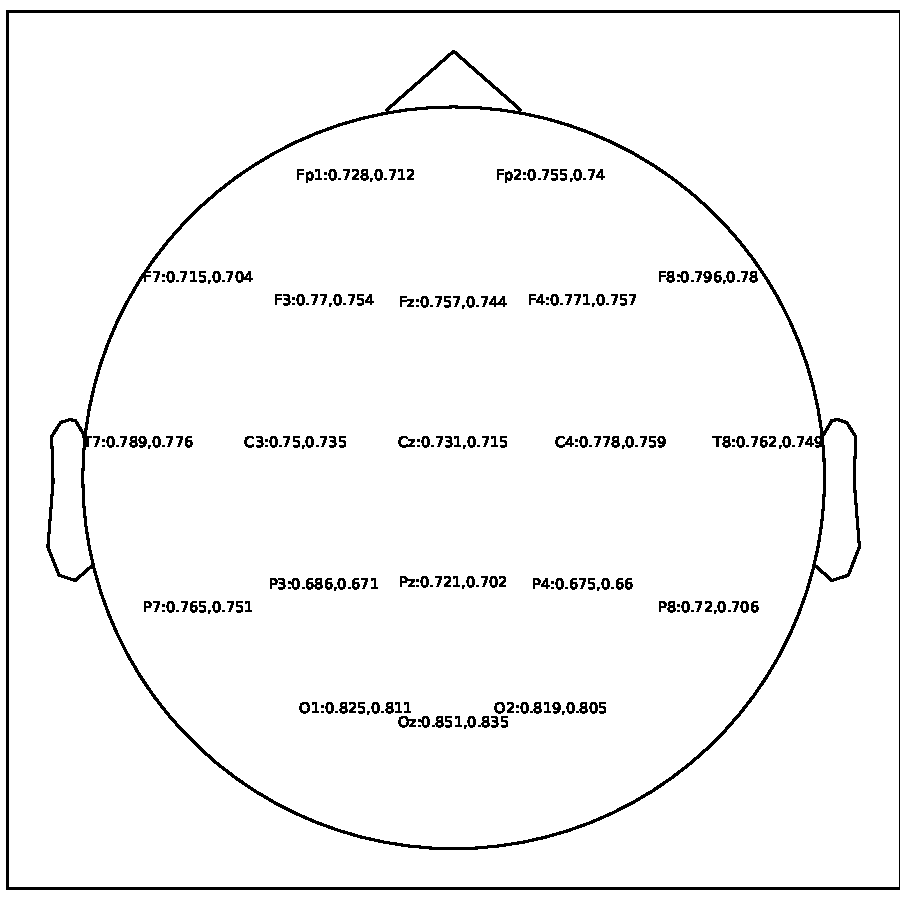
\includegraphics[width=.95\textwidth,trim={0cm 0cm 0cm 0cm},clip]{../SearchResults_1Ch/SearchSpaceResult_1Ch_S109_RemoveBaseLineOff_SamplesIn4Out8_Avg_20191027}};
	  \begin{scope}[scale=1]
	      \draw[line width=2pt,blue] (-7.85,-7.85) node[anchor=west,right=.15cm] {\small{Best Channels according to the train accuracy}} circle (.2);
	      \draw[line width=2pt,red]  (7.85,-7.85)  node[anchor=east,left=.15cm] {\small{Best Channels according to the test accuracy}}  circle (.2);
	      %
	      %\draw[line width=2pt,blue] (-.25,.15) node[] 	(CzTr) {} circle (.45);
	      %\draw[line width=2pt,blue] (-3.2,.15) node[] 	(C3Tr) {} circle (.45);
	      %\draw[line width=2pt,blue] (2.75,.15) node[] 	(C4Tr) {} circle (.45);
	      %\draw[line width=2pt,blue] (-.25, 2.8) node[] 	(FzTr) {} circle (.45);
	      %\draw[line width=2pt,blue] (2.2, 2.85) node[] 	(F4Tr) {} circle (.45);
	      %\draw[line width=2pt,blue] (4.6, 3.25) node[] 	(F8Tr) {} circle (.45);
	      %\draw[line width=2pt,blue] (-2., 5.2) node[] 	(FP1Tr) {} circle (.45);
	      %\draw[line width=2pt,blue] (1.7, 5.2) node[] 	(FP2Tr) {} circle (.45);
	      \draw[line width=2pt,blue] (-.2,-5.1) node[] 	(OzTr) {} circle (.45);
 	      \draw[line width=2pt,blue] (-2.05,-4.85) node[] 	(O1Tr) {} circle (.45);
 	      \draw[line width=2pt,blue] (1.65,-4.85) node[] 	(O2Tr) {} circle (.45);
 	      %\draw[line width=2pt,blue] (-.25, -2.5) node[] 	(PzTr) {} circle (.45);
	      %\draw[line width=2pt,blue] (-2.7, -2.5) node[] 	(P3Tr) {} circle (.45);
	      %\draw[line width=2pt,blue] (-5., -2.95) node[] 	(P7Tr) {} circle (.45);
	      %\draw[line width=2pt,blue] (4.6, -2.95) node[] 	(P8Tr) {} circle (.45);
	      %\draw[line width=2pt,blue] (-6.1,.15) node[] 	(T7Tr) {} circle (.45);
	      %\draw[line width=2pt,blue] (5.75, .15) node[] 	(T8Tr) {} circle (.45);
	      %
	      %\draw[line width=2pt,red] (.65, .15) node[] 	(CzTe) {} circle (.45);
 	      %\draw[line width=2pt,red] (-2.3, .15) node[] 	(C3Te) {} circle (.45);
	      %\draw[line width=2pt,red] (2.8+1, .15) node[] 	(C4Te) {} circle (.45);
	      %\draw[line width=2pt,red] (.6,2.8) node[] 	(FzTe) {} circle (.45);
	      %\draw[line width=2pt,red] (3.1, 2.85) node[] 	(F4Te) {} circle (.45);
	      %\draw[line width=2pt,red] (-4.15, 3.25) node[] 	(F7Te) {} circle (.45);
	      %\draw[line width=2pt,red] (5.45, 3.25) node[] 	(F8Te) {} circle (.45);
	      %\draw[line width=2pt,red] (2.55,5.2) node[] 	(FP2Te) {} circle (.45);
	      \draw[line width=2pt,red] (.7, -5.15) node[] 	(OzTe) {} circle (.45);
	      \draw[line width=2pt,red] (-1.18, -4.85) node[] 	(O1Te) {} circle (.45);
	      \draw[line width=2pt,red] (2.65, -4.85) node[] 	(O2Te) {} circle (.45);
	      %\draw[line width=2pt,red] (.6,-2.5) node[] 	(PzTe) {} circle (.45);
	      %\draw[line width=2pt,red] (3.1,-2.5) node[] 	(P4Te) {} circle (.45);
	      %\draw[line width=2pt,red] (5.45,-2.95) node[] 	(P8Te) {} circle (.45);
	      %\draw[line width=2pt,red] (-5.25, .15) node[] 	(T7Te) {} circle (.45);
 	      %\draw[line width=2pt,red] (6.6, .15) node[] 	(T8Te) {} circle (.45);
	\end{scope}
  \end{tikzpicture}
  \caption{Avg. Results for Searching first best channel with $109$ subjects, no baseline is removed.}
  \label{fg:1Ch_S109_B0_Avg}
\end{figure}

%%%%%%%%%%%%%%%%%%%%%%%%%%%%%%%%%%%%%%%%%%%%%%%%%%%%%%%%%%%%%%%%%%%%%%%%%%%%%%%%%%%%%%%%%%%%%%%%%%%%%%%%%%%
% SearchSpaceResult_2Ch_S109_RemoveBaseLineOff_OrthogonalOn
\newpage
\addtolength{\topmargin}{-.6in}
\hspace*{12cm}\hyperlink{tab:TestResults}{(BACK TO RESULT TABLE)}

\section{Two Channels, With Orthogonalization}

\centerline{
\begin{tabular}{lllll}
  \noalign{\hrule height 2pt}
  No. of Channels: & 2  &&
  No. of Subjects: & 109\\ 
  Previous Selected Channels: & Oz &&
  Baseline Channel: & --\\
  Task:	& REO &&
  No. of Epochs: & 30\\
  Orthogonal:& Yes&&
  Tries:& 10\\
  Inner Shift: & 4 &&
  Outer Shift: & 8\\
  Train Data Percentage: & 80\%&&
  Test Data Percentage: & 20\%\\
  \noalign{\hrule height 2pt}
\end{tabular}}

\bigskip

\begin{table}[!hb]
  \renewcommand{\arraystretch}{1.5}
  \begin{center}
      \caption{Avg. Results for Searching the second best channel with $109$ subjects with orthogonalization. No baseline is removed. Channels are sorted due to the test data accuracy.}
      \label{tab:TestResults}
      \begin{tabular}{c|cc|cc}
	  \noalign{\hrule height 2pt}
	  \mr{2}{\Vasat{.1}{Channel}}& \mc{2}{Train Data}   & \mc{2}{Test Data}\\[.7em]
	  \hhline{~|--|--}
	  & Loss & Acc. & Loss & Acc.\\
	  \hhline{-|--|--}
	  Oz	&	0.1000	&	0.0000	$\pm$	0.0000	&	0.0000	&	0.0000	$\pm$	0.0000	\\
	  C3	&	0.0434	&	0.9859	$\pm$	0.0054	&	0.0566	&	0.9806	$\pm$	0.0060	\\
	  O1	&	0.0511	&	0.9845	$\pm$	0.0239	&	0.0604	&	0.9813	$\pm$	0.0248	\\
	  Cz	&	0.0396	&	0.9872	$\pm$	0.0083	&	0.0508	&	0.9828	$\pm$	0.0089	\\
	  Fp2	&	0.0350	&	0.9889	$\pm$	0.0131	&	0.0475	&	0.9845	$\pm$	0.0147	\\
	  O2	&	0.0372	&	0.9881	$\pm$	0.0103	&	0.0475	&	0.9845	$\pm$	0.0115	\\
	  Pz	&	0.0352	&	0.9889	$\pm$	0.0111	&	0.0466	&	0.9847	$\pm$	0.0119	\\
	  F7	&	0.0342	&	0.9892	$\pm$	0.0098	&	0.0442	&	0.9852	$\pm$	0.0115	\\
	  T7	&	0.0314	&	0.9902	$\pm$	0.0056	&	0.0423	&	0.9862	$\pm$	0.0060	\\
	  F8	&	0.0309	&	0.9903	$\pm$	0.0100	&	0.0411	&	0.9866	$\pm$	0.0123	\\
	  C4	&	0.0307	&	0.9906	$\pm$	0.0073	&	0.0411	&	0.9867	$\pm$	0.0085	\\
	  T8	&	0.0309	&	0.9904	$\pm$	0.0047	&	0.0412	&	0.9869	$\pm$	0.0053	\\
	  P8	&	0.0293	&	0.9909	$\pm$	0.0035	&	0.0393	&	0.9869	$\pm$	0.0041	\\
	  P3	&	0.0318	&	0.9903	$\pm$	0.0090	&	0.0408	&	0.9871	$\pm$	0.0107	\\
	  Fp1	&	0.0287	&	0.9906	$\pm$	0.0115	&	0.0371	&	0.9874	$\pm$	0.0119	\\
	  F3	&	0.0295	&	0.9912	$\pm$	0.0077	&	0.0389	&	0.9874	$\pm$	0.0083	\\
	  Fz	&	0.0299	&	0.9907	$\pm$	0.0070	&	0.0390	&	0.9874	$\pm$	0.0081	\\
	  P7	&	0.0270	&	0.9918	$\pm$	0.0056	&	0.0377	&	0.9878	$\pm$	0.0068	\\
	  P4	&	0.0245	&	0.9926	$\pm$	0.0038	&	0.0344	&	0.9888	$\pm$	0.0042	\\
	  F4	&	0.0200	&	0.9944	$\pm$	0.0034	&	0.0286	&	0.9911	$\pm$	0.0041	\\
	  \noalign{\hrule height 2pt}
      \end{tabular}
  \end{center}

 %%%%%%%%%%%%%%%%%%%%%%%%%%%%%%%%%%%%%%%%%%%%%%%%%%%%%%%%
 %%%%%%%%%%%%%%%%%%%%%%%%%%%%%%%%%%%%%%%%%%%%%%%%%%%%%%%%
 
  \renewcommand{\arraystretch}{1.25}
  \newcommand{\mcl}[2]{\multicolumn{#1}{|c}{#2}}
  \begin{minipage}{1\linewidth} 
      \begin{center}
	\caption{Best channels, in order, in each try.}
	\label{tab:TestResults}
	{\footnotesize
	    \begin{tabular}{p{.3cm}|p{.3cm}||p{.3cm}|p{.3cm}||p{.3cm}|p{.3cm}||p{.3cm}|p{.3cm}||p{.3cm}|p{.3cm}||p{.3cm}|p{.3cm}||p{.3cm}|p{.3cm}||p{.3cm}|p{.3cm}||p{.3cm}|p{.3cm}||p{.3cm}|p{.3cm}}
		\noalign{\hrule height 2pt}
		\mc{2}{Try 1}		&	\mcl{2}{Try 2} 		&	\mcl{2}{Try 3} 		&	\mcl{2}{Try 4} 		&	\mcl{2}{Try 5} 		&	\mcl{2}{Try 6} 		&	\mcl{2}{Try 7} 		&	\mcl{2}{Try 8} 		&	\mcl{2}{Try 9} 		&	\mcl{2}{Try 10}\\
		\hhline{-|-|-|-|-|-|-|-|-|-|-|-|-|-|-|-|-|-|-|-}
		Tr 	& 	Te 	&	Tr 	& 	Te 	&	Tr 	& 	Te	&	Tr 	& 	Te 	&	Tr 	& 	Te	&	Tr 	& 	Te 	&	Tr 	& 	Te 	&	Tr 	& 	Te 	&	Tr 	& 	Te 	&	Tr 	& 	Te\\
		\hhline{-|-|-|-|-|-|-|-|-|-|-|-|-|-|-|-|-|-|-|-}
		P7	&	P7	&	T8	&	O1	&	P7	&	Fp1	&	Fz	&	Fz	&	Fp1	&	Fp1	&	\BB{F4}	&	P3	&	Fz	&	Fz	&	Fp1	&	F8	&	F8	&	F8	&	F3	&	F3\\
		T7	&	T7	&	P4	&	P4	&	Fp1	&	P7	&	Fp1	&	Fp1	&	P7	&	P7	&	P3	&	Fz	&	C4	&	P4	&	F8	&	Fp1	&	F3	&	P3	&	O1	&	O1\\
		F7	&	F7	&	O1	&	T8	&	\BB{F4}	&	\BB{F4}	&	Cz	&	Cz	&	\BB{F4}	&	Fz	&	Fp2	&	Fp1	&	P4	&	C4	&	C4	&	C4	&	P3	&	Fp2	&	\BB{F4}	&	\BB{F4}\\
		P4	&	Fp1	&	O2	&	O2	&	Cz	&	Cz	&	F7	&	F7	&	Fz	&	O2	&	Fz	&	\BB{F4}	&	O1	&	O1	&	\BB{F4}	&	\BB{F4}	&	Fp2	&	\BB{F4}	&	Cz	&	Pz\\
		\BB{F4}	&	Fp1	&	Cz	&	P3	&	F7	&	Pz	&	Fp2	&	Fp2	&	C4	&	\BB{F4}	&	Pz	&	F3	&	P8	&	P7	&	P8	&	P8	&	O1	&	F3	&	Pz	&	F7\\
		\noalign{\hrule height 2pt}
	    \end{tabular}
	}
      \end{center}
  \end{minipage}	
\end{table}


\newpage
\addtolength{\topmargin}{.6in}
{\normalfont\large\bfseries Test Conditions of Case 2:} $^{\text(continued)}$


\bigskip
\bigskip

\centerline{
\begin{tabular}{lllll}
  \noalign{\hrule height 2pt}
  No. of Channels: & 2  &&
  No. of Subjects: & 109\\ 
  Previous Selected Channels: & Oz &&
  Baseline Channel: & --\\
  Task:	& REO &&
  No. of Epochs: & 30\\
  Orthogonal:& Yes&&
  Tries:& 10\\
  Inner Shift: & 4 &&
  Outer Shift: & 8\\
  Train Data Percentage: & 80\%&&
  Test Data Percentage: & 20\%\\
  \noalign{\hrule height 2pt}
\end{tabular}}

\bigskip
\bigskip

\begin{figure}[H]
  \tikzexternaldisable
  \centering
  \begin{tikzpicture}
	  \node[inner sep=0pt] (russell) at (0,0)
	      {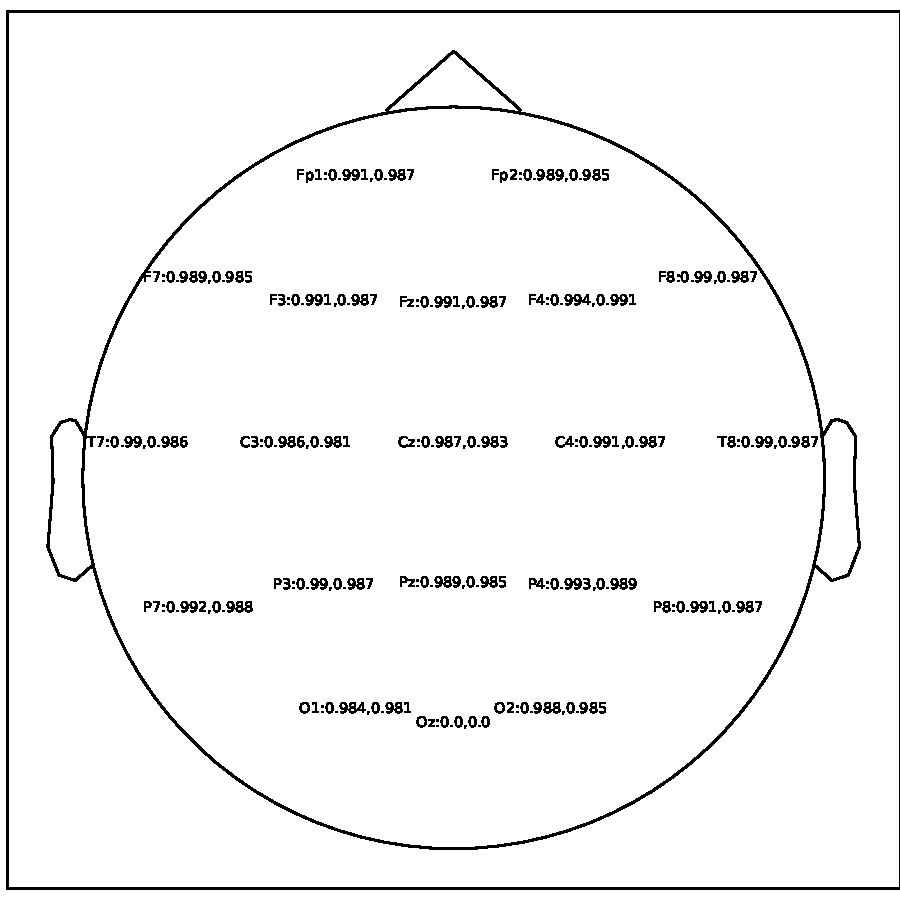
\includegraphics[width=.95\textwidth,trim={0cm 0cm 0cm 0cm},clip]{../SearchResults_2Ch/SearchSpaceResult_2Ch_(61)_S109_RemoveBaseLineOff_OrthogonalOn_SamplesIn4Out8_Avg_E30_20191106}};
	  \begin{scope}[scale=1]
	      \draw[line width=2pt,blue] (-7.85,-7.85) node[anchor=west,right=.15cm] {\small{Best Channels according to the train accuracy}} circle (.2);
	      \draw[line width=2pt,red]  (7.85,-7.85)  node[anchor=east,left=.15cm] {\small{Best Channels according to the test accuracy}}  circle (.2);
	      \draw[line width=2pt,green,fill=green] (-7.15,7.85) node[anchor=west,right=.15cm,opacity=1] {{Previously Selected Channels}} circle (.25);
 	      %
	      \draw[line width=2pt,green,fill=green,opacity=.5] (-.48,-5.15) node[] 	(OzPS) {} circle (.25);
 	      %
	      %\draw[line width=2pt,blue] (-.25,.15) node[] 	(CzTr) {} circle (.45);
	      %\draw[line width=2pt,blue] (-3.2,.15) node[] 	(C3Tr) {} circle (.45);
	      %\draw[line width=2pt,blue] (2.75,.15) node[] 	(C4Tr) {} circle (.45);
	      %\draw[line width=2pt,blue] (-.2, 2.8) node[] 	(FzTr) {} circle (.45);
	      \draw[line width=2pt,blue] (2.2, 2.85) node[] 	(F4Tr) {} circle (.45);
	      %\draw[line width=2pt,blue] (4.75, 3.25) node[] 	(F8Tr) {} circle (.45);
	      %\draw[line width=2pt,blue] (-2., 5.2) node[] 	(FP1Tr) {} circle (.45);
	      %\draw[line width=2pt,blue] (1.7, 5.2) node[] 	(FP2Tr) {} circle (.45);
	      %\draw[line width=2pt,blue] (-.2,-5.1) node[] 	(OzTr) {} circle (.45);
 	      %\draw[line width=2pt,blue] (-2.05,-4.85) node[] 	(O1Tr) {} circle (.45);
 	      %\draw[line width=2pt,blue] (1.65,-4.85) node[] 	(O2Tr) {} circle (.45);
 	      %\draw[line width=2pt,blue] (-.25, -2.5) node[] 	(PzTr) {} circle (.45);
	      %\draw[line width=2pt,blue] (-2.7, -2.5) node[] 	(P3Tr) {} circle (.45);
	      \draw[line width=2pt,blue] (2.4, -2.5) node[] 	(P4Tr) {} circle (.45);
	      \draw[line width=2pt,blue] (-5., -2.95) node[] 	(P7Tr) {} circle (.45);
	      %\draw[line width=2pt,blue] (4.7, -2.95) node[] 	(P8Tr) {} circle (.45);
	      %\draw[line width=2pt,blue] (-6.1,.15) node[] 	(T7Tr) {} circle (.45);
	      %\draw[line width=2pt,blue] (5.75, .15) node[] 	(T8Tr) {} circle (.45);
	      %
	      %\draw[line width=2pt,red] (.65, .15) node[] 	(CzTe) {} circle (.45);
 	      %\draw[line width=2pt,red] (-2.3, .15) node[] 	(C3Te) {} circle (.45);
	      %\draw[line width=2pt,red] (2.8+1, .15) node[] 	(C4Te) {} circle (.45);
	      %\draw[line width=2pt,red] (.65,2.8) node[] 	(FzTe) {} circle (.45);
	      \draw[line width=2pt,red] (3.1, 2.85) node[] 	(F4Te) {} circle (.45);
	      %\draw[line width=2pt,red] (-4.15, 3.25) node[] 	(F7Te) {} circle (.45);
	      %\draw[line width=2pt,red] (5.55, 3.25) node[] 	(F8Te) {} circle (.45);
	      %\draw[line width=2pt,red] (-1., 5.2) node[] 	(FP1Te) {} circle (.45);
	      %\draw[line width=2pt,red] (2.55,5.2) node[] 	(FP2Te) {} circle (.45);
	      %\draw[line width=2pt,red] (.7, -5.15) node[] 	(OzTe) {} circle (.45);
	      %\draw[line width=2pt,red] (-1.18, -4.85) node[] 	(O1Te) {} circle (.45);
	      %\draw[line width=2pt,red] (2.65, -4.85) node[] 	(O2Te) {} circle (.45);
	      %\draw[line width=2pt,red] (.6,-2.5) node[] 	(PzTe) {} circle (.45);
	      \draw[line width=2pt,red] (3.1,-2.5) node[] 	(P4Te) {} circle (.45);
	      \draw[line width=2pt,red] (-4.2, -2.95) node[] 	(P7Te) {} circle (.45);
	      %\draw[line width=2pt,red] (5.55,-2.95) node[] 	(P8Te) {} circle (.45);
	      %\draw[line width=2pt,red] (-5.25, .15) node[] 	(T7Te) {} circle (.45);
 	      %\draw[line width=2pt,red] (6.6, .15) node[] 	(T8Te) {} circle (.45);
	\end{scope}
  \end{tikzpicture}
  \caption{Avg. Results for Searching the second best channel with $109$ subjects with orthogonalization. No baseline is removed.}
  \label{fg:2Ch_S109_B0_Ort1_Avg}
\end{figure}

%%%%%%%%%%%%%%%%%%%%%%%%%%%%%%%%%%%%%%%%%%%%%%%%%%%%%%%%%%%%%%%%%%%%%%%%%%%%%%%%%%%%%%%%%%%%%%%%%%%%%%%%%%%
% SearchSpaceResult_2Ch_S109_RemoveBaseLineOff_OrthogonalOff
\newpage
\addtolength{\topmargin}{-.6in}
\hspace*{12cm}\hyperlink{tab:TestResults}{(BACK TO RESULT TABLE)}

\section{Two Channels, Without Orthogonalization}

\centerline{
\begin{tabular}{lllll}
  \noalign{\hrule height 2pt}
  No. of Channels: & 2  &&
  No. of Subjects: & 109\\ 
  Previous Selected Channels: & Oz &&
  Baseline Channel: & --\\
  Task:	& REO &&
  No. of Epochs: & 30\\
  Orthogonal:& No&&
  Tries:& 10\\
  Inner Shift: & 4 &&
  Outer Shift: & 8\\
  Train Data Percentage: & 80\%&&
  Test Data Percentage: & 20\%\\
  \noalign{\hrule height 2pt}
\end{tabular}}

\bigskip

\begin{table}[!hb]
  \renewcommand{\arraystretch}{1.5}
  \begin{center}
      \caption{Avg. Results for Searching the second best channel with $109$ subjects Without orthogonalization. No baseline is removed. Channels are sorted due to the test data accuracy.}
      \label{tab:TestResults}
      \begin{tabular}{c|cc|cc}
	  \noalign{\hrule height 2pt}
	  \mr{2}{\Vasat{.1}{Channel}}& \mc{2}{Train Data}   & \mc{2}{Test Data}\\[.7em]
	  \hhline{~|--|--}
	  & Loss & Acc. & Loss & Acc.\\
	  \hhline{-|--|--}
	  Oz	&	0.1000	&	0.0000	$\pm$	0.0000	&	0.0000	&	0.0000	$\pm$	0.0000	\\
	  P8	&	0.1373	&	0.9557	$\pm$	0.0368	&	0.1613	&	0.9476	$\pm$	0.0379	\\
	  P4	&	0.1221	&	0.9618	$\pm$	0.0374	&	0.1451	&	0.9536	$\pm$	0.0389	\\
	  P3	&	0.1003	&	0.9681	$\pm$	0.0203	&	0.1235	&	0.9595	$\pm$	0.0208	\\
	  O1	&	0.0980	&	0.9672	$\pm$	0.0159	&	0.1181	&	0.9598	$\pm$	0.0164	\\
	  Fp2	&	0.0963	&	0.9705	$\pm$	0.0158	&	0.1227	&	0.9608	$\pm$	0.0187	\\
	  Cz	&	0.0982	&	0.9694	$\pm$	0.0184	&	0.1184	&	0.9617	$\pm$	0.0195	\\
	  T7	&	0.0995	&	0.9681	$\pm$	0.0303	&	0.1175	&	0.9618	$\pm$	0.0298	\\
	  C3	&	0.0936	&	0.9713	$\pm$	0.0166	&	0.1151	&	0.9633	$\pm$	0.0176	\\
	  O2	&	0.0872	&	0.9713	$\pm$	0.0136	&	0.1072	&	0.9640	$\pm$	0.0148	\\
	  T8	&	0.0913	&	0.9715	$\pm$	0.0192	&	0.1091	&	0.9649	$\pm$	0.0211	\\
	  F3	&	0.0844	&	0.9732	$\pm$	0.0176	&	0.1025	&	0.9658	$\pm$	0.0196	\\
	  Fp1	&	0.0852	&	0.9744	$\pm$	0.0189	&	0.1085	&	0.9659	$\pm$	0.0199	\\
	  P7	&	0.0810	&	0.9744	$\pm$	0.0122	&	0.1030	&	0.9661	$\pm$	0.0129	\\
	  C4	&	0.0886	&	0.9728	$\pm$	0.0194	&	0.1073	&	0.9664	$\pm$	0.0206	\\
	  Pz	&	0.0828	&	0.9748	$\pm$	0.0104	&	0.1027	&	0.9667	$\pm$	0.0118	\\
	  F7	&	0.0753	&	0.9778	$\pm$	0.0071	&	0.0960	&	0.9694	$\pm$	0.0086	\\
	  F4	&	0.0674	&	0.9784	$\pm$	0.0172	&	0.0848	&	0.9717	$\pm$	0.0194	\\
	  Fz	&	0.0615	&	0.9814	$\pm$	0.0078	&	0.0781	&	0.9751	$\pm$	0.0086	\\
	  F8	&	0.0627	&	0.9810	$\pm$	0.0081	&	0.0767	&	0.9751	$\pm$	0.0086	\\
	  \noalign{\hrule height 2pt}
      \end{tabular}
  \end{center}

 %%%%%%%%%%%%%%%%%%%%%%%%%%%%%%%%%%%%%%%%%%%%%%%%%%%%%%%%
 %%%%%%%%%%%%%%%%%%%%%%%%%%%%%%%%%%%%%%%%%%%%%%%%%%%%%%%%
 
  \renewcommand{\arraystretch}{1.25}
  \newcommand{\mcl}[2]{\multicolumn{#1}{|c}{#2}}
  \begin{minipage}{1\linewidth} 
      \begin{center}
	\caption{Best channels, in order, in each try.}
	\label{tab:TestResults}
	{\footnotesize
	    \begin{tabular}{p{.3cm}|p{.3cm}||p{.3cm}|p{.3cm}||p{.3cm}|p{.3cm}||p{.3cm}|p{.3cm}||p{.3cm}|p{.3cm}||p{.3cm}|p{.3cm}||p{.3cm}|p{.3cm}||p{.3cm}|p{.3cm}||p{.3cm}|p{.3cm}||p{.3cm}|p{.3cm}}
		\noalign{\hrule height 2pt}
		\mc{2}{Try 1}		&	\mcl{2}{Try 2} 		&	\mcl{2}{Try 3} 		&	\mcl{2}{Try 4} 		&	\mcl{2}{Try 5} 		&	\mcl{2}{Try 6} 		&	\mcl{2}{Try 7} 		&	\mcl{2}{Try 8} 		&	\mcl{2}{Try 9} 		&	\mcl{2}{Try 10}\\
		\hhline{-|-|-|-|-|-|-|-|-|-|-|-|-|-|-|-|-|-|-|-}
		Tr 	& 	Te 	&	Tr 	& 	Te 	&	Tr 	& 	Te	&	Tr 	& 	Te 	&	Tr 	& 	Te	&	Tr 	& 	Te 	&	Tr 	& 	Te 	&	Tr 	& 	Te 	&	Tr 	& 	Te 	&	Tr 	& 	Te\\
		\hhline{-|-|-|-|-|-|-|-|-|-|-|-|-|-|-|-|-|-|-|-}
		O2	&	O2	&	Fz	&	F4	&	F4	&	F4	&	T8	&	T8	&	Fp1	&	Fp1	&	F4	&	F4	&	P4	&	P4	&	T7	&	T7	&	T7	&	T7	&	T8	&	F3	\\
		Fp1	&	Fp1	&	F4	&	Fz	&	\BB{F8}	&	\BB{F8}	&	Cz	&	Cz	&	T7	&	T8	&	C4	&	P3	&	C3	&	Fp1	&	F4	&	P8	&	C4	&	C4	&	F3	&	T8	\\
		F4	&	F4	&	F3	&	F3	&	C3	&	Fz	&	O2	&	O2	&	T8	&	T7	&	\BB{F8}	&	F4	&	Fz	&	\BB{F8}	&	Fz	&	F4	&	P7	&	P7	&	F7	&	\BB{F8}	\\
		O1	&	O1	&	P4	&	P4	&	Fz	&	C3	&	O1	&	Fz	&	\BB{F8}	&	Fz	&	Fp2	&	Cz	&	Fp1	&	C3	&	P8	&	O2	&	C3	&	\BB{F8}	&	\BB{F8}	&	F7	\\
		P4	&	C4	&	\BB{F8}	&	\BB{F8}	&	Cz	&	F7	&	Fz	&	O1	&	C4	&	\BB{F8}	&	Pz	&	Fp1	&	\BB{F8}	&	T8	&	P3	&	Fz	&	\BB{F8}	&	C3	&	Pz	&	Cz	\\
		\noalign{\hrule height 2pt}
	    \end{tabular}
	}
      \end{center}
  \end{minipage}	
\end{table}


\newpage
\addtolength{\topmargin}{.6in}
{\normalfont\large\bfseries Test Conditions of Case 3:} $^{\text(continued)}$


\bigskip
\bigskip

\centerline{
\begin{tabular}{lllll}
  \noalign{\hrule height 2pt}
  No. of Channels: & 2  &&
  No. of Subjects: & 109\\ 
  Previous Selected Channels: & Oz &&
  Baseline Channel: & --\\
  Task:	& REO &&
  No. of Epochs: & 30\\
  Orthogonal:& No&&
  Tries:& 10\\
  Inner Shift: & 4 &&
  Outer Shift: & 8\\
  Train Data Percentage: & 80\%&&
  Test Data Percentage: & 20\%\\
  \noalign{\hrule height 2pt}
\end{tabular}}

\bigskip
\bigskip

\begin{figure}[H]
  \tikzexternaldisable
  \centering
  \begin{tikzpicture}
	  \node[inner sep=0pt] (russell) at (0,0)
	      {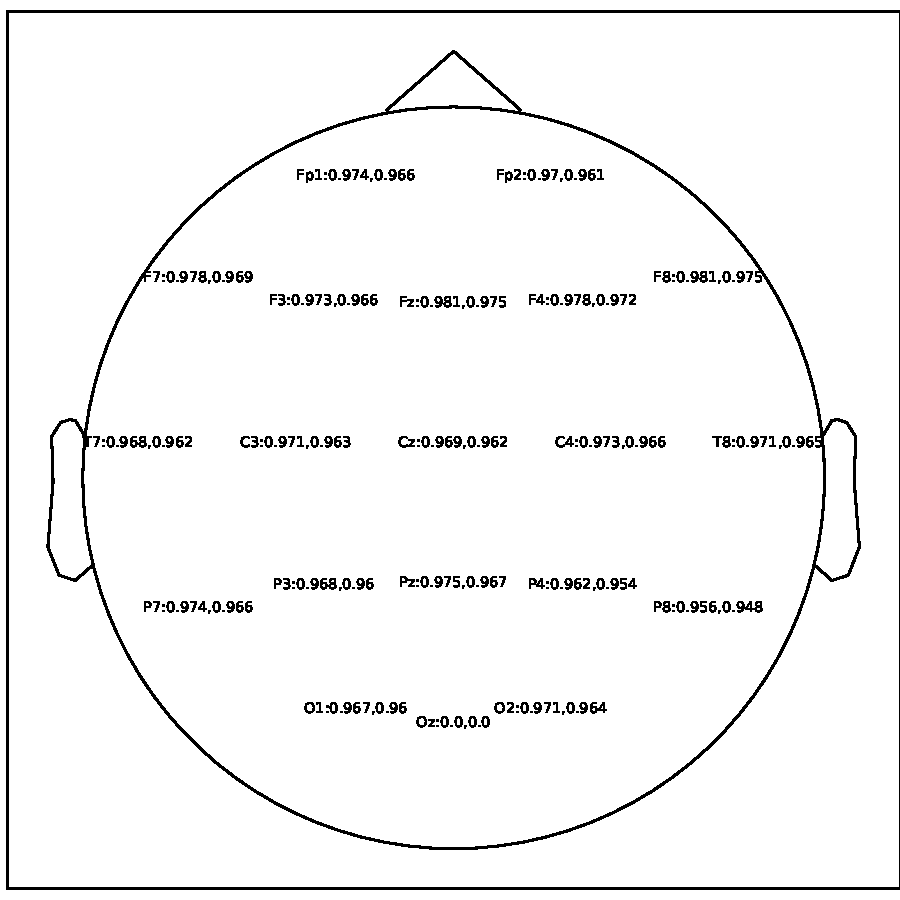
\includegraphics[width=.95\textwidth,trim={0cm 0cm 0cm 0cm},clip]{../SearchResults_2Ch/SearchSpaceResult_2Ch_(61)_S109_RemoveBaseLineOff_OrthogonalOff_SamplesIn4Out8_Avg_E30_20191106}};
	  \begin{scope}[scale=1]
	      \draw[line width=2pt,blue] (-7.85,-7.85) node[anchor=west,right=.15cm] {\small{Best Channels according to the train accuracy}} circle (.2);
	      \draw[line width=2pt,red]  (7.85,-7.85)  node[anchor=east,left=.15cm] {\small{Best Channels according to the test accuracy}}  circle (.2);
	      \draw[line width=2pt,green,fill=green] (-7.15,7.85) node[anchor=west,right=.15cm,opacity=1] {{Previously Selected Channels}} circle (.25);
 	      %
	      \draw[line width=2pt,green,fill=green,opacity=.5] (-.48,-5.15) node[] 	(OzPS) {} circle (.25);
 	      %
	      %\draw[line width=2pt,blue] (-.25,.15) node[] 	(CzTr) {} circle (.45);
	      %\draw[line width=2pt,blue] (-3.2,.15) node[] 	(C3Tr) {} circle (.45);
	      %\draw[line width=2pt,blue] (2.75,.15) node[] 	(C4Tr) {} circle (.45);
	      \draw[line width=2pt,blue] (-.2, 2.8) node[] 	(FzTr) {} circle (.45);
	      \draw[line width=2pt,blue] (2.2, 2.85) node[] 	(F4Tr) {} circle (.45);
	      \draw[line width=2pt,blue] (4.75, 3.25) node[] 	(F8Tr) {} circle (.45);
	      %\draw[line width=2pt,blue] (-2., 5.2) node[] 	(FP1Tr) {} circle (.45);
	      %\draw[line width=2pt,blue] (1.7, 5.2) node[] 	(FP2Tr) {} circle (.45);
	      %\draw[line width=2pt,blue] (-.2,-5.1) node[] 	(OzTr) {} circle (.45);
 	      %\draw[line width=2pt,blue] (-2.05,-4.85) node[] 	(O1Tr) {} circle (.45);
 	      %\draw[line width=2pt,blue] (1.65,-4.85) node[] 	(O2Tr) {} circle (.45);
 	      %\draw[line width=2pt,blue] (-.25, -2.5) node[] 	(PzTr) {} circle (.45);
	      %\draw[line width=2pt,blue] (-2.7, -2.5) node[] 	(P3Tr) {} circle (.45);
	      %\draw[line width=2pt,blue] (2.4, -2.5) node[] 	(P4Tr) {} circle (.45);
	      %\draw[line width=2pt,blue] (-5., -2.95) node[] 	(P7Tr) {} circle (.45);
	      %\draw[line width=2pt,blue] (4.7, -2.95) node[] 	(P8Tr) {} circle (.45);
	      %\draw[line width=2pt,blue] (-6.1,.15) node[] 	(T7Tr) {} circle (.45);
	      %\draw[line width=2pt,blue] (5.75, .15) node[] 	(T8Tr) {} circle (.45);
	      %
	      %\draw[line width=2pt,red] (.65, .15) node[] 	(CzTe) {} circle (.45);
 	      %\draw[line width=2pt,red] (-2.3, .15) node[] 	(C3Te) {} circle (.45);
	      %\draw[line width=2pt,red] (2.8+1, .15) node[] 	(C4Te) {} circle (.45);
	      \draw[line width=2pt,red] (.65,2.8) node[] 	(FzTe) {} circle (.45);
	      \draw[line width=2pt,red] (3.1, 2.85) node[] 	(F4Te) {} circle (.45);
	      %\draw[line width=2pt,red] (-4.15, 3.25) node[] 	(F7Te) {} circle (.45);
	      \draw[line width=2pt,red] (5.55, 3.25) node[] 	(F8Te) {} circle (.45);
	      %\draw[line width=2pt,red] (-1., 5.2) node[] 	(FP1Te) {} circle (.45);
	      %\draw[line width=2pt,red] (2.55,5.2) node[] 	(FP2Te) {} circle (.45);
	      %\draw[line width=2pt,red] (.7, -5.15) node[] 	(OzTe) {} circle (.45);
	      %\draw[line width=2pt,red] (-1.18, -4.85) node[] 	(O1Te) {} circle (.45);
	      %\draw[line width=2pt,red] (2.65, -4.85) node[] 	(O2Te) {} circle (.45);
	      %\draw[line width=2pt,red] (.6,-2.5) node[] 	(PzTe) {} circle (.45);
	      %\draw[line width=2pt,red] (3.1,-2.5) node[] 	(P4Te) {} circle (.45);
	      %\draw[line width=2pt,red] (-4.2, -2.95) node[] 	(P7Te) {} circle (.45);
	      %\draw[line width=2pt,red] (5.55,-2.95) node[] 	(P8Te) {} circle (.45);
	      %\draw[line width=2pt,red] (-5.25, .15) node[] 	(T7Te) {} circle (.45);
 	      %\draw[line width=2pt,red] (6.6, .15) node[] 	(T8Te) {} circle (.45);
	\end{scope}
  \end{tikzpicture}
  \caption{Avg. Results for Searching the second best channel with $109$ subjects without orthogonalization. No baseline is removed.}
  \label{fg:2Ch_S109_B0_Ort0_Avg}
\end{figure}

%%%%%%%%%%%%%%%%%%%%%%%%%%%%%%%%%%%%%%%%%%%%%%%%%%%%%%%%%%%%%%%%%%%%%%%%%%%%%%%%%%%%%%%%%%%%%%%%%%%%%%%%%%%
% SearchSpaceResult_3Ch_S109_RemoveBaseLineOff_OrthogonalOn
\newpage
\addtolength{\topmargin}{-.6in}
\hspace*{12cm}\hyperlink{tab:TestResults}{(BACK TO RESULT TABLE)}

\section{Three Channels, With Orthogonalization}

\centerline{
\begin{tabular}{lllll}
  \noalign{\hrule height 2pt}
  No. of Channels: & 3  &&
  No. of Subjects: & 109\\ 
  Previous Selected Channels: & Oz, F4 &&
  Baseline Channel: & --\\
  Task:	& REO &&
  No. of Epochs: & 30\\
  Orthogonal:& Yes&&
  Tries:& 11\\
  Inner Shift: & 4 &&
  Outer Shift: & 8\\
  Train Data Percentage: & 80\%&&
  Test Data Percentage: & 20\%\\
  \noalign{\hrule height 2pt}
\end{tabular}}

\bigskip

\begin{table}[!hb]
  \renewcommand{\arraystretch}{1.5}
  \begin{center}
      \caption{Avg. Results for Searching the third best channel with $109$ subjects with orthogonalization. No baseline is removed. Channels are sorted due to the test data accuracy.}
      \label{tab:TestResults}
      \begin{tabular}{c|cc|cc}
	  \noalign{\hrule height 2pt}
	  \mr{2}{\Vasat{.1}{Channel}}& \mc{2}{Train Data}   & \mc{2}{Test Data}\\[.7em]
	  \hhline{~|--|--}
	  & Loss & Acc. & Loss & Acc.\\
	  \hhline{-|--|--}
	  F4	&	0.1000	&	0.0000	$\pm$	0.0000	&	0.0000	&	0.0000	$\pm$	0.0000	\\
	  Oz	&	0.1000	&	0.0000	$\pm$	0.0000	&	0.0000	&	0.0000	$\pm$	0.0000	\\
	  P8	&	0.0119	&	0.9964	$\pm$	0.0052	&	0.0165	&	0.9949	$\pm$	0.0062	\\
	  F8	&	0.0105	&	0.9967	$\pm$	0.0050	&	0.0135	&	0.9957	$\pm$	0.0058	\\
	  O1	&	0.0087	&	0.9973	$\pm$	0.0040	&	0.0125	&	0.9960	$\pm$	0.0021	\\
	  P3	&	0.0089	&	0.9972	$\pm$	0.0030	&	0.0126	&	0.9960	$\pm$	0.0039	\\
	  Fp2	&	0.0083	&	0.9974	$\pm$	0.0023	&	0.0116	&	0.9962	$\pm$	0.0030	\\
	  Cz	&	0.0089	&	0.9972	$\pm$	0.0035	&	0.0121	&	0.9962	$\pm$	0.0045	\\
	  T8	&	0.0085	&	0.9974	$\pm$	0.0033	&	0.0110	&	0.9966	$\pm$	0.0029	\\
	  Pz	&	0.0072	&	0.9978	$\pm$	0.0022	&	0.0104	&	0.9967	$\pm$	0.0028	\\
	  F7	&	0.0066	&	0.9981	$\pm$	0.0012	&	0.0101	&	0.9969	$\pm$	0.0017	\\
	  T7	&	0.0076	&	0.9978	$\pm$	0.0021	&	0.0104	&	0.9969	$\pm$	0.0026	\\
	  F3	&	0.0063	&	0.9982	$\pm$	0.0011	&	0.0094	&	0.9970	$\pm$	0.0016	\\
	  C3	&	0.0073	&	0.9979	$\pm$	0.0030	&	0.0097	&	0.9971	$\pm$	0.0038	\\
	  P7	&	0.0064	&	0.9981	$\pm$	0.0016	&	0.0092	&	0.9971	$\pm$	0.0015	\\
	  Fz	&	0.0057	&	0.9982	$\pm$	0.0012	&	0.0082	&	0.9973	$\pm$	0.0015	\\
	  C4	&	0.0060	&	0.9982	$\pm$	0.0014	&	0.0083	&	0.9974	$\pm$	0.0014	\\
	  O2	&	0.0057	&	0.9984	$\pm$	0.0012	&	0.0085	&	0.9975	$\pm$	0.0017	\\
	  P4	&	0.0059	&	0.9984	$\pm$	0.0016	&	0.0083	&	0.9975	$\pm$	0.0018	\\
	  Fp1	&	0.0052	&	0.9984	$\pm$	0.0016	&	0.0072	&	0.9976	$\pm$	0.0020	\\
	  \noalign{\hrule height 2pt}
      \end{tabular}
  \end{center}

 %%%%%%%%%%%%%%%%%%%%%%%%%%%%%%%%%%%%%%%%%%%%%%%%%%%%%%%%
 %%%%%%%%%%%%%%%%%%%%%%%%%%%%%%%%%%%%%%%%%%%%%%%%%%%%%%%%
 
  \renewcommand{\arraystretch}{1.25}
  \newcommand{\mcl}[2]{\multicolumn{#1}{|c}{#2}}
  \begin{minipage}{1\linewidth} 
      \begin{center}
	\caption{Best channels, in order, in each try.}
	\label{tab:TestResults}
	{\footnotesize
	    \begin{tabular}{p{.3cm}|p{.3cm}||p{.3cm}|p{.3cm}||p{.3cm}|p{.3cm}||p{.3cm}|p{.3cm}||p{.3cm}|p{.3cm}||p{.3cm}|p{.3cm}||p{.3cm}|p{.3cm}||p{.3cm}|p{.3cm}||p{.3cm}|p{.3cm}||p{.3cm}|p{.3cm}||p{.3cm}|p{.3cm}}
		\noalign{\hrule height 2pt}
		\mc{2}{Try 1}		&	\mcl{2}{Try 2} 		&	\mcl{2}{Try 3} 		&	\mcl{2}{Try 4} 		&	\mcl{2}{Try 5} 		&	\mcl{2}{Try 6} 		&	\mcl{2}{Try 7} 		&	\mcl{2}{Try 8} 		&	\mcl{2}{Try 9} 		&	\mcl{2}{Try 10}		&	\mcl{2}{Try 11}		\\
		\hhline{-|-|-|-|-|-|-|-|-|-|-|-|-|-|-|-|-|-|-|-|-|-}
		Tr 	& 	Te 	&	Tr 	& 	Te 	&	Tr 	& 	Te	&	Tr 	& 	Te 	&	Tr 	& 	Te	&	Tr 	& 	Te 	&	Tr 	& 	Te 	&	Tr 	& 	Te 	&	Tr 	& 	Te 	&	Tr 	& 	Te	&	Tr 	& 	Te	\\
		\hhline{-|-|-|-|-|-|-|-|-|-|-|-|-|-|-|-|-|-|-|-|-|-}
		C4	&	C4	&	C3	&	O2	&	P7	&	P7	&	T8	&	T8	&	\BB{Fp1}&	\BB{Fp1}&	O1	&	T7	&	\BB{Fp1}&	\BB{Fp1}&	T7	&	T7	&	Fz	&	Fz	&	F8	&	F8	&	Cz	&	Cz	\\
		F8	&	Fp2	&	O2	&	C3	&	P4	&	Pz	&	Fz	&	Fz	&	P8	&	P8	&	Cz	&	F8	&	C4	&	C4	&	P3	&	Pz	&	F8	&	Fz	&	P7	&	T8	&	O2	&	F7	\\
		Fp2	&	F8	&	Cz	&	Cz	&	O1	&	P4	&	F3	&	C3	&	C3	&	C3	&	T7	&	F7	&	P8	&	C3	&	Pz	&	P3	&	O2	&	F7	&	T8	&	P7	&	F7	&	O2	\\
		T8	&	T8	&	C4	&	T7	&	Pz	&	Cz	&	T7	&	C3	&	Pz	&	Pz	&	T8	&	C4	&	T7	&	Fz	&	C3	&	C3	&	O1	&	O1	&	F3	&	Fp2	&	\BB{Fp1}&	\BB{Fp1}\\
		P4	&	T8	&	C4	&	T8	&	Cz	&	O2	&	Pz	&	Pz	&	T7	&	Pz	&	C3	&	T7	&	Fp2	&	Fz	&	F7	&	P4	&	F7	&	\BB{Fp1}&	Fp2	&	F3	&	Fp2	&	\BB{Fp1}\\
		\noalign{\hrule height 2pt}
	    \end{tabular}
	}
      \end{center}
  \end{minipage}	
\end{table}


\newpage
\addtolength{\topmargin}{.6in}
{\normalfont\large\bfseries Test Conditions of Case 4:} $^{\text(continued)}$


\bigskip
\bigskip

\centerline{
\begin{tabular}{lllll}
  \noalign{\hrule height 2pt}
  No. of Channels: & 3  &&
  No. of Subjects: & 109\\ 
  Previous Selected Channels: & Oz, F4 &&
  Baseline Channel: & --\\
  Task:	& REO &&
  No. of Epochs: & 30\\
  Orthogonal:& Yes&&
  Tries:& 11\\
  Inner Shift: & 4 &&
  Outer Shift: & 8\\
  Train Data Percentage: & 80\%&&
  Test Data Percentage: & 20\%\\
  \noalign{\hrule height 2pt}
\end{tabular}}

\bigskip
\bigskip

\begin{figure}[H]
  \tikzexternaldisable
  \centering
  \begin{tikzpicture}
	  \node[inner sep=0pt] (russell) at (0,0)
	      {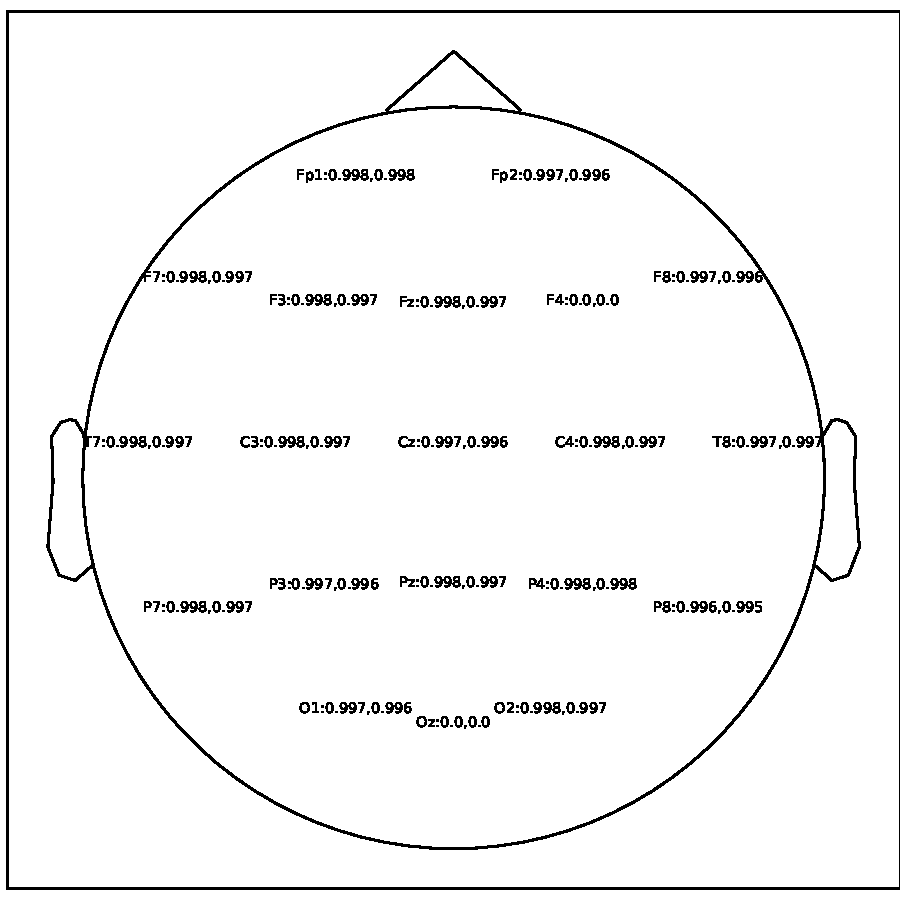
\includegraphics[width=.95\textwidth,trim={0cm 0cm 0cm 0cm},clip]{../SearchResults_3Ch/SearchSpaceResult_3Ch_(61_33)_S109_RemoveBaseLineOff_OrthogonalOn_SamplesIn4Out8_Avg_E30_20191111_20191112}};
	  \begin{scope}[scale=1]
	      \draw[line width=2pt,blue] (-7.85,-7.85) node[anchor=west,right=.15cm] {\small{Best Channels according to the train accuracy}} circle (.2);
	      \draw[line width=2pt,red]  (7.85,-7.85)  node[anchor=east,left=.15cm] {\small{Best Channels according to the test accuracy}}  circle (.2);
	      \draw[line width=2pt,green,fill=green] (-7.15,7.85) node[anchor=west,right=.15cm,opacity=1] {{Previously Selected Channels}} circle (.25);
 	      %
	      \draw[line width=2pt,green,fill=green,opacity=.5] (-.48,-5.15) node[] 	(OzPS) {} circle (.25);
 	      \draw[line width=2pt,green,fill=green,opacity=.5] (2,2.85) node[] 	(F4PS) {} circle (.25);
 	      %
	      %\draw[line width=2pt,blue] (-.25,.15) node[] 	(CzTr) {} circle (.45);
	      %\draw[line width=2pt,blue] (-3.2,.15) node[] 	(C3Tr) {} circle (.45);
	      %\draw[line width=2pt,blue] (2.75,.15) node[] 	(C4Tr) {} circle (.45);
	      %\draw[line width=2pt,blue] (-.2, 2.8) node[] 	(FzTr) {} circle (.45);
	      %\draw[line width=2pt,blue] (2.2, 2.85) node[] 	(F4Tr) {} circle (.45);
	      %\draw[line width=2pt,blue] (4.75, 3.25) node[] 	(F8Tr) {} circle (.45);
	      \draw[line width=2pt,blue] (-1.9, 5.25) node[] 	(FP1Tr) {} circle (.45);
	      %\draw[line width=2pt,blue] (1.7, 5.2) node[] 	(FP2Tr) {} circle (.45);
	      %\draw[line width=2pt,blue] (-.2,-5.1) node[] 	(OzTr) {} circle (.45);
 	      %\draw[line width=2pt,blue] (-2.05,-4.85) node[] 	(O1Tr) {} circle (.45);
 	      \draw[line width=2pt,blue] (1.65,-4.85) node[] 	(O2Tr) {} circle (.45);
 	      %\draw[line width=2pt,blue] (-.25, -2.5) node[] 	(PzTr) {} circle (.45);
	      %\draw[line width=2pt,blue] (-2.7, -2.5) node[] 	(P3Tr) {} circle (.45);
	      \draw[line width=2pt,blue] (2.3, -2.5) node[] 	(P4Tr) {} circle (.45);
	      %\draw[line width=2pt,blue] (-5., -2.95) node[] 	(P7Tr) {} circle (.45);
	      %\draw[line width=2pt,blue] (4.7, -2.95) node[] 	(P8Tr) {} circle (.45);
	      %\draw[line width=2pt,blue] (-6.1,.15) node[] 	(T7Tr) {} circle (.45);
	      %\draw[line width=2pt,blue] (5.75, .15) node[] 	(T8Tr) {} circle (.45);
	      %
	      %\draw[line width=2pt,red] (.65, .15) node[] 	(CzTe) {} circle (.45);
 	      %\draw[line width=2pt,red] (-2.3, .15) node[] 	(C3Te) {} circle (.45);
	      %\draw[line width=2pt,red] (2.8+1, .15) node[] 	(C4Te) {} circle (.45);
	      %\draw[line width=2pt,red] (.65,2.8) node[] 	(FzTe) {} circle (.45);
	      %\draw[line width=2pt,red] (3.1, 2.85) node[] 	(F4Te) {} circle (.45);
	      %\draw[line width=2pt,red] (-4.15, 3.25) node[] 	(F7Te) {} circle (.45);
	      %\draw[line width=2pt,red] (5.55, 3.25) node[] 	(F8Te) {} circle (.45);
	      \draw[line width=2pt,red] (-1.1, 5.25) node[] 	(FP1Te) {} circle (.45);
	      %\draw[line width=2pt,red] (2.55,5.2) node[] 	(FP2Te) {} circle (.45);
	      %\draw[line width=2pt,red] (.7, -5.15) node[] 	(OzTe) {} circle (.45);
	      %\draw[line width=2pt,red] (-1.18, -4.85) node[] 	(O1Te) {} circle (.45);
	      \draw[line width=2pt,red] (2.65, -4.85) node[] 	(O2Te) {} circle (.45);
	      %\draw[line width=2pt,red] (.6,-2.5) node[] 	(PzTe) {} circle (.45);
	      \draw[line width=2pt,red] (3.2,-2.5) node[] 	(P4Te) {} circle (.45);
	      %\draw[line width=2pt,red] (-4.2, -2.95) node[] 	(P7Te) {} circle (.45);
	      %\draw[line width=2pt,red] (5.55,-2.95) node[] 	(P8Te) {} circle (.45);
	      %\draw[line width=2pt,red] (-5.25, .15) node[] 	(T7Te) {} circle (.45);
 	      %\draw[line width=2pt,red] (6.6, .15) node[] 	(T8Te) {} circle (.45);
	\end{scope}
  \end{tikzpicture}
  \caption{Avg. Results for Searching the third best channel with $109$ subjects with orthogonalization. No baseline is removed.}
  \label{fg:3Ch_S109_B0_Ort1_Avg}
\end{figure}

%%%%%%%%%%%%%%%%%%%%%%%%%%%%%%%%%%%%%%%%%%%%%%%%%%%%%%%%%%%%%%%%%%%%%%%%%%%%%%%%%%%%%%%%%%%%%%%%%%%%%%%%%%%
% SearchSpaceResult_3Ch_S109_RemoveBaseLineOff_OrthogonalOff
\newpage
\addtolength{\topmargin}{-.6in}
\hspace*{12cm}\hyperlink{tab:TestResults}{(BACK TO RESULT TABLE)}

\section{Three Channels, Without Orthogonalization}

\centerline{
\begin{tabular}{lllll}
  \noalign{\hrule height 2pt}
  No. of Channels: & 3  &&
  No. of Subjects: & 109\\ 
  Previous Selected Channels: & Oz, Fz &&
  Baseline Channel: & --\\
  Task:	& REO &&
  No. of Epochs: & 30\\
  Orthogonal:& No&&
  Tries:& 10\\
  Inner Shift: & 4 &&
  Outer Shift: & 8\\
  Train Data Percentage: & 80\%&&
  Test Data Percentage: & 20\%\\
  \noalign{\hrule height 2pt}
\end{tabular}}

\bigskip

\begin{table}[!hb]
  \renewcommand{\arraystretch}{1.5}
  \begin{center}
      \caption{Avg. Results for Searching the third best channel with $109$ subjects without orthogonalization. No baseline is removed. Channels are sorted due to the test data accuracy.}
      \label{tab:TestResults}
      \begin{tabular}{c|cc|cc}
	  \noalign{\hrule height 2pt}
	  \mr{2}{\Vasat{.1}{Channel}}& \mc{2}{Train Data}   & \mc{2}{Test Data}\\[.7em]
	  \hhline{~|--|--}
	  & Loss & Acc. & Loss & Acc.\\
	  \hhline{-|--|--}
	  Fz	&	0.1000	&	0.0000	$\pm$	0.0000	&	0.0000	&	0.0000	$\pm$	0.0000	\\
	  Oz	&	0.1000	&	0.0000	$\pm$	0.0000	&	0.0000	&	0.0000	$\pm$	0.0000	\\
	  C4	&	0.0622	&	0.9794	$\pm$	0.0152	&	0.0764	&	0.9742	$\pm$	0.0169	\\
	  F7	&	0.0623	&	0.9800	$\pm$	0.0175	&	0.0767	&	0.9750	$\pm$	0.0201	\\
	  Pz	&	0.0590	&	0.9809	$\pm$	0.0156	&	0.0729	&	0.9760	$\pm$	0.0172	\\
	  Fp2	&	0.0516	&	0.9841	$\pm$	0.0165	&	0.0643	&	0.9793	$\pm$	0.0177	\\
	  P4	&	0.0463	&	0.9854	$\pm$	0.0111	&	0.0593	&	0.9804	$\pm$	0.0125	\\
	  Fp1	&	0.0482	&	0.9855	$\pm$	0.0081	&	0.0617	&	0.9806	$\pm$	0.0088	\\
	  C3	&	0.0450	&	0.9858	$\pm$	0.0097	&	0.0587	&	0.9808	$\pm$	0.0109	\\
	  P7	&	0.0448	&	0.9860	$\pm$	0.0084	&	0.0576	&	0.9811	$\pm$	0.0091	\\
	  O1	&	0.0459	&	0.9856	$\pm$	0.0108	&	0.0586	&	0.9811	$\pm$	0.0114	\\
	  Cz	&	0.0413	&	0.9878	$\pm$	0.0097	&	0.0535	&	0.9830	$\pm$	0.0110	\\
	  F8	&	0.0417	&	0.9871	$\pm$	0.0174	&	0.0515	&	0.9832	$\pm$	0.0193	\\
	  T7	&	0.0430	&	0.9871	$\pm$	0.0156	&	0.0540	&	0.9832	$\pm$	0.0176	\\
	  P3	&	0.0408	&	0.9879	$\pm$	0.0147	&	0.0527	&	0.9832	$\pm$	0.0168	\\
	  T8	&	0.0425	&	0.9868	$\pm$	0.0191	&	0.0531	&	0.9833	$\pm$	0.0216	\\
	  F3	&	0.0375	&	0.9891	$\pm$	0.0082	&	0.0483	&	0.9849	$\pm$	0.0089	\\
	  P8	&	0.0350	&	0.9900	$\pm$	0.0067	&	0.0457	&	0.9861	$\pm$	0.0079	\\
	  F4	&	0.0353	&	0.9908	$\pm$	0.0061	&	0.0459	&	0.9869	$\pm$	0.0070	\\
	  O2	&	0.0214	&	0.9940	$\pm$	0.0035	&	0.0298	&	0.9906	$\pm$	0.0041	\\
	  \noalign{\hrule height 2pt}
      \end{tabular}
  \end{center}

 %%%%%%%%%%%%%%%%%%%%%%%%%%%%%%%%%%%%%%%%%%%%%%%%%%%%%%%%
 %%%%%%%%%%%%%%%%%%%%%%%%%%%%%%%%%%%%%%%%%%%%%%%%%%%%%%%%
 
  \renewcommand{\arraystretch}{1.25}
  \newcommand{\mcl}[2]{\multicolumn{#1}{|c}{#2}}
  \begin{minipage}{1\linewidth} 
      \begin{center}
	\caption{Best channels, in order, in each try.}
	\label{tab:TestResults}
	{\footnotesize
	    \begin{tabular}{p{.3cm}|p{.3cm}||p{.3cm}|p{.3cm}||p{.3cm}|p{.3cm}||p{.3cm}|p{.3cm}||p{.3cm}|p{.3cm}||p{.3cm}|p{.3cm}||p{.3cm}|p{.3cm}||p{.3cm}|p{.3cm}||p{.3cm}|p{.3cm}||p{.3cm}|p{.3cm}}
		\noalign{\hrule height 2pt}
		\mc{2}{Try 1}		&	\mcl{2}{Try 2} 		&	\mcl{2}{Try 3} 		&	\mcl{2}{Try 4} 		&	\mcl{2}{Try 5} 		&	\mcl{2}{Try 6} 		&	\mcl{2}{Try 7} 		&	\mcl{2}{Try 8} 		&	\mcl{2}{Try 9} 		&	\mcl{2}{Try 10}		\\
		\hhline{-|-|-|-|-|-|-|-|-|-|-|-|-|-|-|-|-|-|-}
		Tr 	& 	Te 	&	Tr 	& 	Te 	&	Tr 	& 	Te	&	Tr 	& 	Te 	&	Tr 	& 	Te	&	Tr 	& 	Te 	&	Tr 	& 	Te 	&	Tr 	& 	Te 	&	Tr 	& 	Te 	&	Tr 	& 	Te	\\
		\hhline{-|-|-|-|-|-|-|-|-|-|-|-|-|-|-|-|-|-|-}
		T7	&	T7	&	F3	&	T8	&	T8	&	T8	&	F8	&	F8	&	C3	&	T8	&	\BB{O2}	&	F8	&	F8	&	F8	&	C4	&	C4	&	T8	&	T8	&	\BB{O2}	&	T8	\\
		O1	&	\BB{O2}	&	T7	&	F4	&	P3	&	P4	&	T8	&	\BB{O2}	&	T8	&	C3	&	F8	&	Oz	&	C3	&	C3	&	P8	&	P8	&	\BB{O2}	&	\BB{O2}	&	T8	&	\BB{O2}	\\
		\BB{O2}	&	O1	&	F4	&	T7	&	P4	&	P3	&	\BB{O2}	&	T8	&	F7	&	P8	&	Fp2	&	Fp1	&	P3	&	P3	&	P7	&	F4	&	P3	&	P3	&	P3	&	P3	\\
		Cz	&	Cz	&	T8	&	F3	&	Fp2	&	T7	&	F4	&	Fp2	&	T7	&	T7	&	F7	&	Fp2	&	Fp1	&	Fp1	&	F4	&	P7	&	Fp2	&	Fp2	&	F3	&	F7	\\
		Pz	&	F8	&	P3	&	P3	&	Cz	&	Fp2	&	Fp2	&	F4	&	P8	&	F7	&	P7	&	T8	&	P8	&	P8	&	\BB{O2}	&	\BB{O2}	&	C4	&	C4	&	P4	&	P4	\\
		\noalign{\hrule height 2pt}
	    \end{tabular}
	}
      \end{center}
  \end{minipage}	
\end{table}


\newpage
\addtolength{\topmargin}{.6in}
{\normalfont\large\bfseries Test Conditions of Case 5:} $^{\text(continued)}$


\bigskip
\bigskip

\centerline{
\begin{tabular}{lllll}
  \noalign{\hrule height 2pt}
  No. of Channels: & 3  &&
  No. of Subjects: & 109\\ 
  Previous Selected Channels: & Oz, Fz &&
  Baseline Channel: & --\\
  Task:	& REO &&
  No. of Epochs: & 30\\
  Orthogonal:& No&&
  Tries:& 10\\
  Inner Shift: & 4 &&
  Outer Shift: & 8\\
  Train Data Percentage: & 80\%&&
  Test Data Percentage: & 20\%\\
  \noalign{\hrule height 2pt}
\end{tabular}}

\bigskip
\bigskip

\begin{figure}[H]
  \tikzexternaldisable
  \centering
  \begin{tikzpicture}
	  \node[inner sep=0pt] (russell) at (0,0)
	      {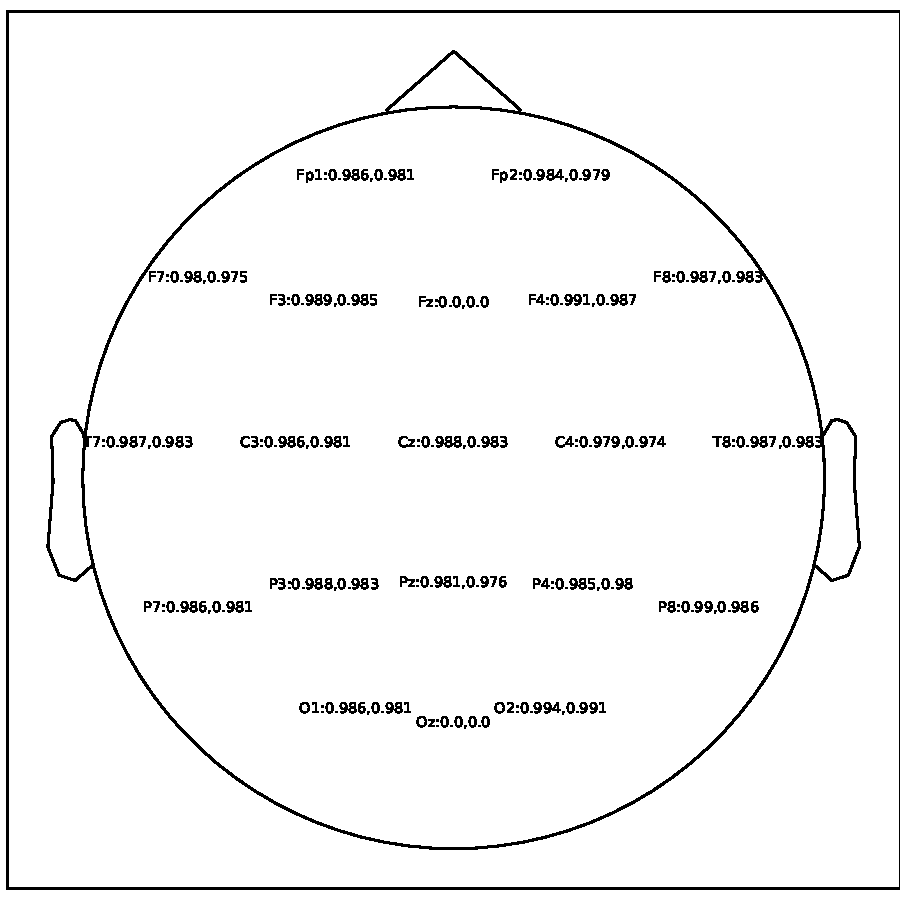
\includegraphics[width=.95\textwidth,trim={0cm 0cm 0cm 0cm},clip]{../SearchResults_3Ch/SearchSpaceResult_3Ch_(61_33)_S109_RemoveBaseLineOff_OrthogonalOff_SamplesIn4Out8_Avg_E30_20191111_20191112}};
	  \begin{scope}[scale=1]
	      \draw[line width=2pt,blue] (-7.85,-7.85) node[anchor=west,right=.15cm] {\small{Best Channels according to the train accuracy}} circle (.2);
	      \draw[line width=2pt,red]  (7.85,-7.85)  node[anchor=east,left=.15cm] {\small{Best Channels according to the test accuracy}}  circle (.2);
	      \draw[line width=2pt,green,fill=green] (-7.15,7.85) node[anchor=west,right=.15cm,opacity=1] {{Previously Selected Channels}} circle (.25);
 	      %
	      \draw[line width=2pt,green,fill=green,opacity=.5] (-.48,-5.15) node[] 	(OzPS) {} circle (.25);
 	      %\draw[line width=2pt,green,fill=green,opacity=.5] (2,2.85) node[] 	(F4PS) {} circle (.25);
 	      \draw[line width=2pt,green,fill=green,opacity=.5] (-.6,2.85) node[] 	(FzPS) {} circle (.25);
 	      %
	      %\draw[line width=2pt,blue] (-.25,.15) node[] 	(CzTr) {} circle (.45);
	      %\draw[line width=2pt,blue] (-3.2,.15) node[] 	(C3Tr) {} circle (.45);
	      %\draw[line width=2pt,blue] (2.75,.15) node[] 	(C4Tr) {} circle (.45);
	      %\draw[line width=2pt,blue] (-.2, 2.8) node[] 	(FzTr) {} circle (.45);
	      \draw[line width=2pt,blue] (2.2, 2.85) node[] 	(F4Tr) {} circle (.45);
	      %\draw[line width=2pt,blue] (4.75, 3.25) node[] 	(F8Tr) {} circle (.45);
	      %\draw[line width=2pt,blue] (-1.9, 5.25) node[] 	(FP1Tr) {} circle (.45);
	      %\draw[line width=2pt,blue] (1.7, 5.2) node[] 	(FP2Tr) {} circle (.45);
	      %\draw[line width=2pt,blue] (-.2,-5.1) node[] 	(OzTr) {} circle (.45);
 	      %\draw[line width=2pt,blue] (-2.05,-4.85) node[] 	(O1Tr) {} circle (.45);
 	      \draw[line width=2pt,blue] (1.65,-4.85) node[] 	(O2Tr) {} circle (.45);
 	      %\draw[line width=2pt,blue] (-.25, -2.5) node[] 	(PzTr) {} circle (.45);
	      %\draw[line width=2pt,blue] (-2.7, -2.5) node[] 	(P3Tr) {} circle (.45);
	      %\draw[line width=2pt,blue] (2.3, -2.5) node[] 	(P4Tr) {} circle (.45);
	      %\draw[line width=2pt,blue] (-5., -2.95) node[] 	(P7Tr) {} circle (.45);
	      \draw[line width=2pt,blue] (4.7, -2.95) node[] 	(P8Tr) {} circle (.45);
	      %\draw[line width=2pt,blue] (-6.1,.15) node[] 	(T7Tr) {} circle (.45);
	      %\draw[line width=2pt,blue] (5.75, .15) node[] 	(T8Tr) {} circle (.45);
	      %
	      %\draw[line width=2pt,red] (.65, .15) node[] 	(CzTe) {} circle (.45);
 	      %\draw[line width=2pt,red] (-2.3, .15) node[] 	(C3Te) {} circle (.45);
	      %\draw[line width=2pt,red] (2.8+1, .15) node[] 	(C4Te) {} circle (.45);
	      %\draw[line width=2pt,red] (.65,2.8) node[] 	(FzTe) {} circle (.45);
	      \draw[line width=2pt,red] (3.1, 2.85) node[] 	(F4Te) {} circle (.45);
	      %\draw[line width=2pt,red] (-4.15, 3.25) node[] 	(F7Te) {} circle (.45);
	      %\draw[line width=2pt,red] (5.55, 3.25) node[] 	(F8Te) {} circle (.45);
	      %\draw[line width=2pt,red] (-1.1, 5.25) node[] 	(FP1Te) {} circle (.45);
	      %\draw[line width=2pt,red] (2.55,5.2) node[] 	(FP2Te) {} circle (.45);
	      %\draw[line width=2pt,red] (.7, -5.15) node[] 	(OzTe) {} circle (.45);
	      %\draw[line width=2pt,red] (-1.18, -4.85) node[] 	(O1Te) {} circle (.45);
	      \draw[line width=2pt,red] (2.65, -4.85) node[] 	(O2Te) {} circle (.45);
	      %\draw[line width=2pt,red] (.6,-2.5) node[] 	(PzTe) {} circle (.45);
	      %\draw[line width=2pt,red] (3.2,-2.5) node[] 	(P4Te) {} circle (.45);
	      %\draw[line width=2pt,red] (-4.2, -2.95) node[] 	(P7Te) {} circle (.45);
	      \draw[line width=2pt,red] (5.55,-2.95) node[] 	(P8Te) {} circle (.45);
	      %\draw[line width=2pt,red] (-5.25, .15) node[] 	(T7Te) {} circle (.45);
 	      %\draw[line width=2pt,red] (6.6, .15) node[] 	(T8Te) {} circle (.45);
	\end{scope}
  \end{tikzpicture}
  \caption{Avg. Results for Searching the third best channel with $109$ subjects without orthogonalization. No baseline is removed.}
  \label{fg:3Ch_S109_B0_Ort1_Avg}
\end{figure}


\end{document}